\clearpage
\section{Impact on nuclear PDFs}
\label{sec:nuclearPDFs}

The study presented in Sect.~\ref{sec:protonPDFs} treated, from the point of view
of PDF constraints, the neutrino scattering target
as composed by isoscalar free-nucleons, and hence neglecting nuclear modifications
and non-isoscalar effects.
%
We now revisit this analysis but accounting for the fact that the target materials in the FPF
experiments actually
composed by heavy nuclei, specifically by tungsten (the exception is FLArE with liquid argon, which
is however not considered here).
%
Nuclear modifications associated to a tungsten target are not necessarily small as compared
to a free isoscalar nucleon, and hence will affect the event rate predictions for
the FPF experiments.
%
Turning the argument around, measurements of differential neutrino cross-sections
on heavy nuclear targets provide direct constraints on these nuclear modifications
without replying on assumptions on the $A$ dependence.

For this exercise, the prior nuclear PDF set is taken to be EPPS21, a global determination
that accounts for the constraints of existing datasets involving nuclei as target or projectiles.
%
In particular, EPPS21 already includes information from neutrino DIS on nuclear targets
from the CHORUS and NuTeV experiments.
%
The application of Hessian profiling to EPPS21 follows the same strategy as that
for PDF4LHC21, with the caveat that its Hessian error sets also include the contribution
from the uncertainties  associated to their reference proton PDF set, in this case CT18.
%
Given that the measured event rates depend on both the proton PDFs and the nuclear modifications,
when profiling EPPS21 we also account for the Hessian sets associated to the CT18 proton
PDF dependence.

Fig.~\ref{fig:profiling_baseline_nuclear} displays the baseline result of the profiling using the EPPS21 global determination of nuclear PDFs,
specifically of the set with $A=184$ (tungsten target).
%
Also in this case we consider first the impact of the baseline LHC neutrino dataset, consisting
on the FASER$\nu$2 experiment
with statistical errors only, inclusive and charm structure functions,  and charge flavour
separation.
%
The bands indicate the 68\% CL uncertainties.

{\color{red}
The effect of including correlated systematic uncertainties is shown in 
Fig.~\ref{fig:profiling_syst_nuclear}
}


%%%%%%%%%%%%%%%%%%%%%%%%%%%%%%%%%%%%%%%%%%%%%%%%%%%%%%%%%%%%%%%%%%%%%5
\begin{figure}[t]
\centering
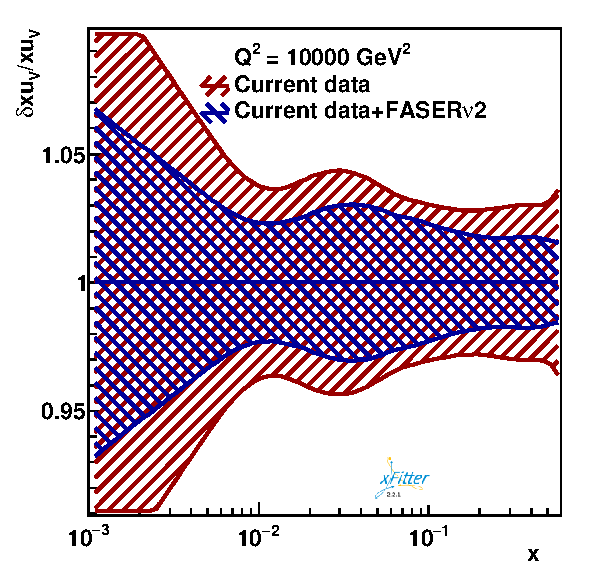
\includegraphics[width=0.32\textwidth]{plots/nuclear_fasernu2/inclusive+charm_chargediscrimination/statOnly_FASERv2_q2_10000_pdf_uv_ratio.pdf}
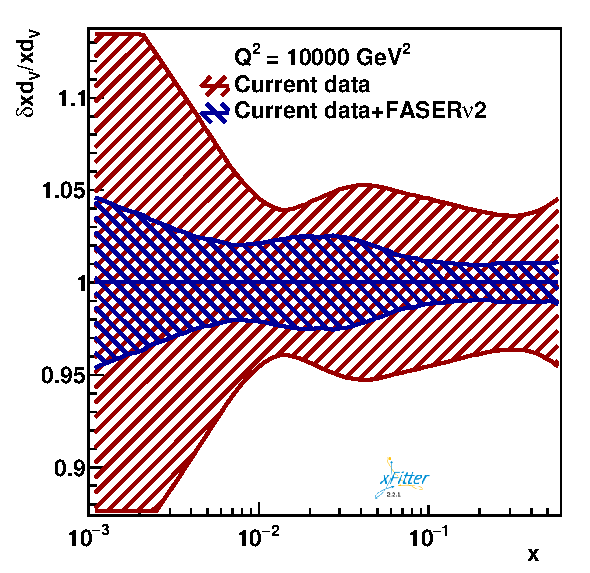
\includegraphics[width=0.32\textwidth]{plots/nuclear_fasernu2/inclusive+charm_chargediscrimination/statOnly_FASERv2_q2_10000_pdf_dv_ratio.pdf}
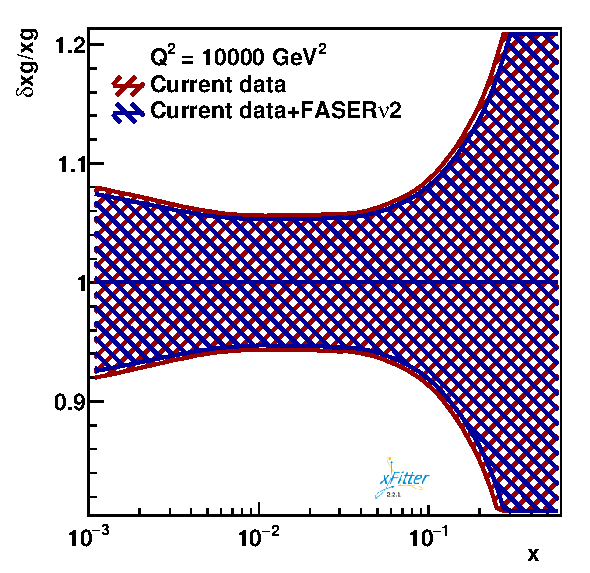
\includegraphics[width=0.32\textwidth]{plots/nuclear_fasernu2/inclusive+charm_chargediscrimination/statOnly_FASERv2_q2_10000_pdf_g_ratio.pdf}\\
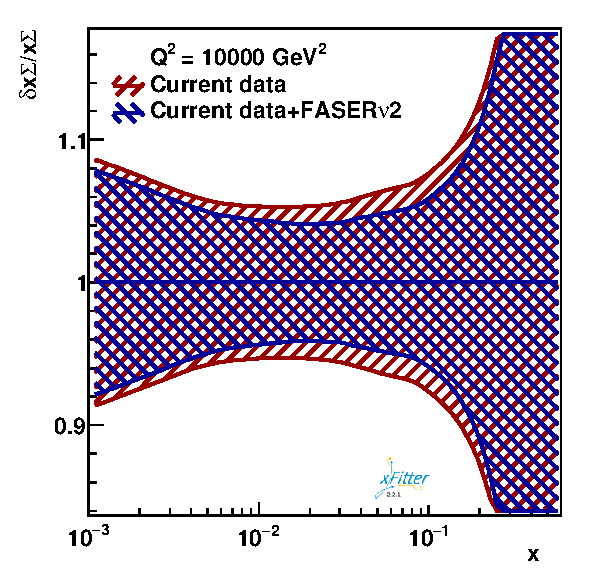
\includegraphics[width=0.32\textwidth]{plots/nuclear_fasernu2/inclusive+charm_chargediscrimination/statOnly_FASERv2_q2_10000_pdf_Sea_ratio.pdf}
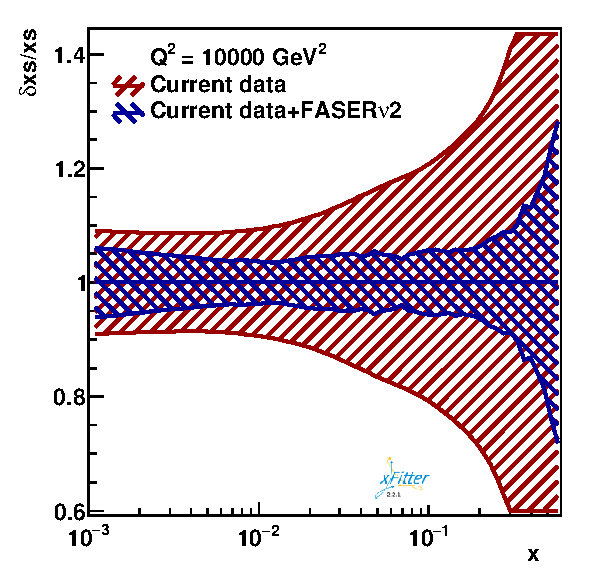
\includegraphics[width=0.32\textwidth]{plots/nuclear_fasernu2/inclusive+charm_chargediscrimination/statOnly_FASERv2_q2_10000_pdf_s_ratio.pdf}
\caption{The fractional uncertainties (90\% confidence level) at $Q^2 = 10^4 \, \textrm{GeV}^2$ of the EPPS21 global determination of nuclear PDFs,
specifically of the set with $A=184$ (tungsten target), compared to the results of profiling with the FASER$\nu$2 DIS projections.
%
Also in this case we consider first the impact of the baseline LHC neutrino dataset, consisting
on the FASER$\nu$2 experiment
with statistical errors only, inclusive and charm structure functions,  and charge flavour
separation.
%
}
\label{fig:profiling_baseline_nuclear}
\end{figure}
%%%%%%%%%%%%%%%%%%%%%%%%%%%%%%%%%%%%%%%%%%%%%%%%%%%%%%%%%%%%%%%%%%%%%%%%
%%%%%%%%%%%%%%%%%%%%%%%%%%%%%%%%%%%%%%%%%%%%%%%%%%%%%%%%%%%%%%%%%%%%%%%%
\begin{figure}[t]
\centering
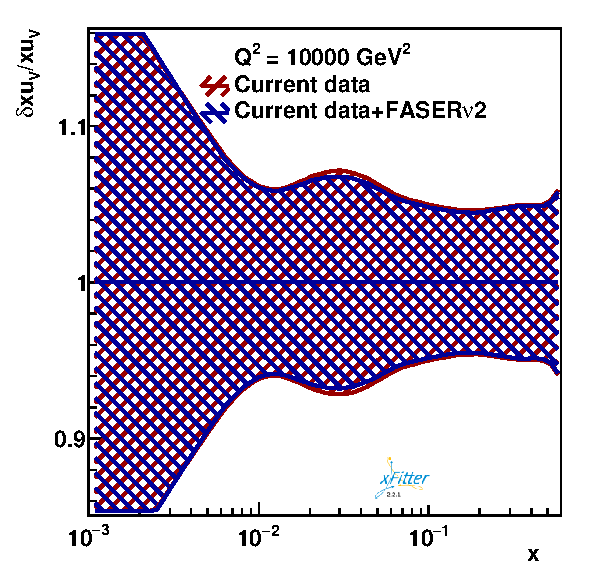
\includegraphics[width=0.32\textwidth]{plots/nuclear_fasernu2/inclusive+charm_chargediscrimination/systVar05_FASERv2_q2_10000_pdf_uv_ratio.pdf}
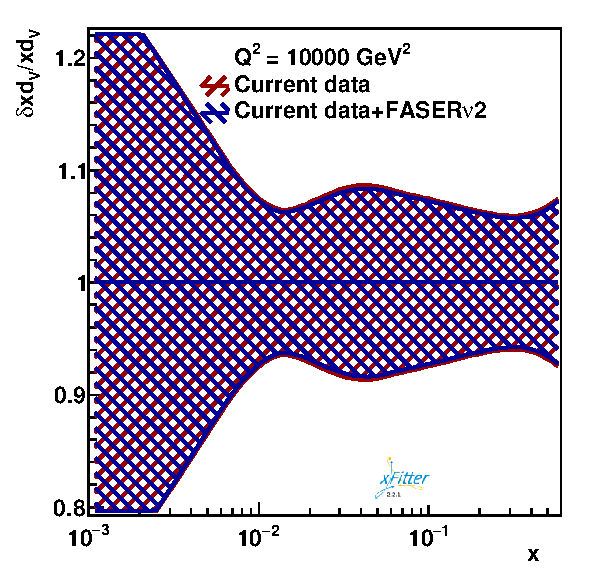
\includegraphics[width=0.32\textwidth]{plots/nuclear_fasernu2/inclusive+charm_chargediscrimination/systVar05_FASERv2_q2_10000_pdf_dv_ratio.pdf}
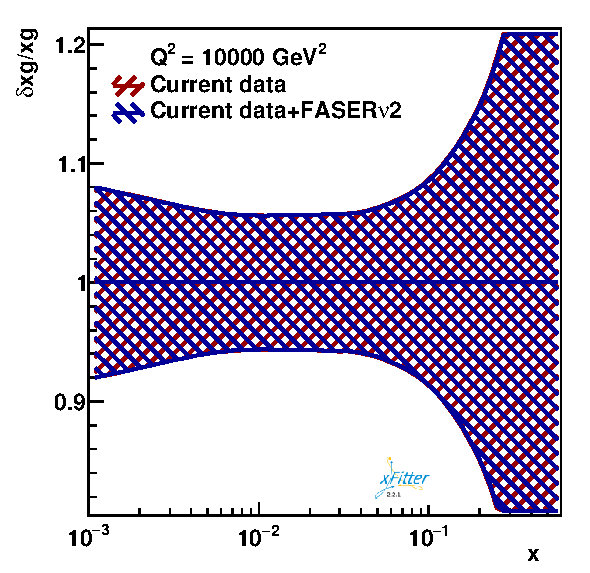
\includegraphics[width=0.32\textwidth]{plots/nuclear_fasernu2/inclusive+charm_chargediscrimination/systVar05_FASERv2_q2_10000_pdf_g_ratio.pdf}\\
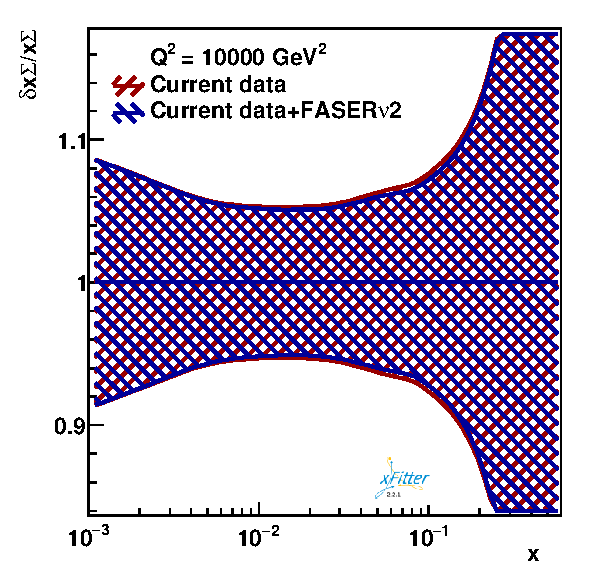
\includegraphics[width=0.32\textwidth]{plots/nuclear_fasernu2/inclusive+charm_chargediscrimination/systVar05_FASERv2_q2_10000_pdf_Sea_ratio.pdf}
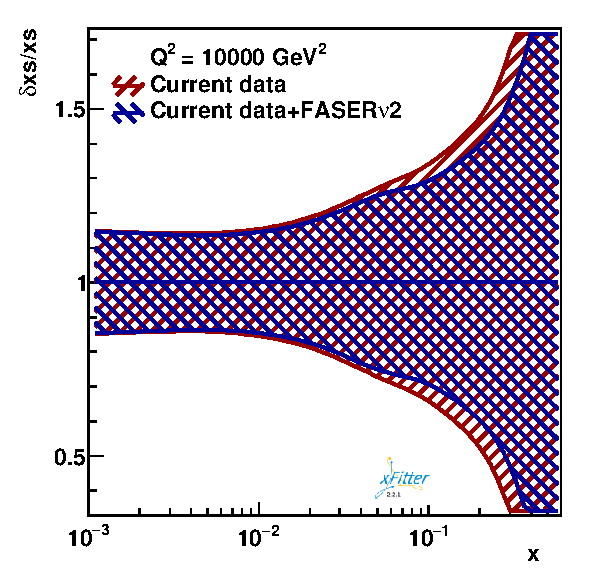
\includegraphics[width=0.32\textwidth]{plots/nuclear_fasernu2/inclusive+charm_chargediscrimination/systVar05_FASERv2_q2_10000_pdf_s_ratio.pdf}
\caption{The results of Fig.~\ref{fig:profiling_baseline_nuclear} (red and blue), 
compared to profiling with the statistical as well as correlated systematic uncertainties accounted for.
}
\label{fig:profiling_syst_nuclear}
\end{figure}
%%%%%%%%%%%%%%%%%%%%%%%%%%%%%%%%%%%%%%%%%%%%%%%%%%%%%%%%%%%%%%%%%%%%%%%%
%%%%%%%%%%%%%%%%%%%%%%%%%%%%%%%%%%%%%%%%%%%%%%%%%%%%%%%%%%%%%%%%%%%%%%%%
\begin{figure}[t]
\centering
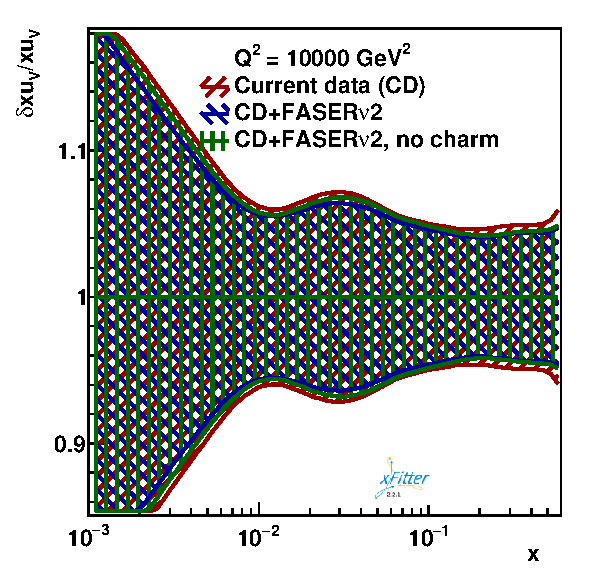
\includegraphics[width=0.32\textwidth]{plots/nuclear_fasernu2/inclusive-only_vs_inclusive+charm/statOnly_FASERv2_q2_10000_pdf_uv_ratio.pdf}
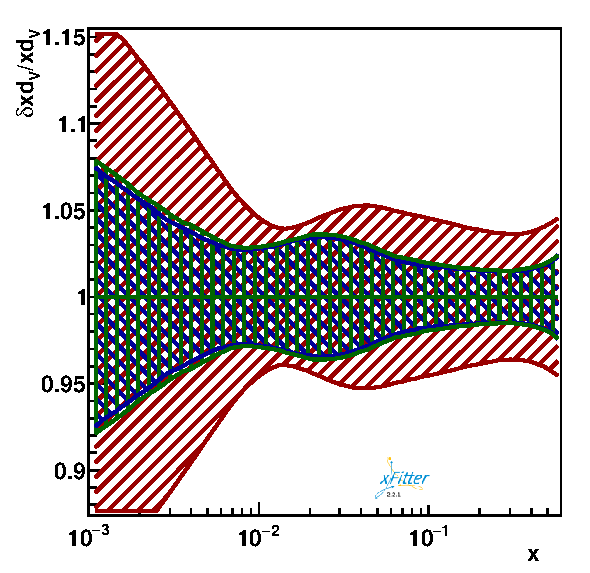
\includegraphics[width=0.32\textwidth]{plots/nuclear_fasernu2/inclusive-only_vs_inclusive+charm/statOnly_FASERv2_q2_10000_pdf_dv_ratio.pdf}
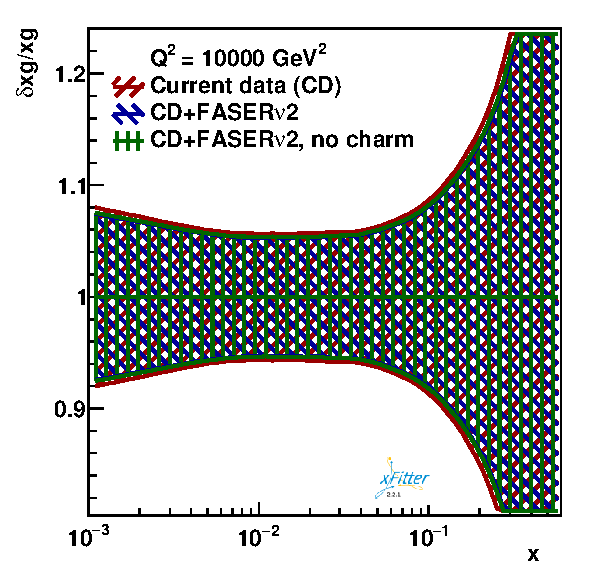
\includegraphics[width=0.32\textwidth]{plots/nuclear_fasernu2/inclusive-only_vs_inclusive+charm/statOnly_FASERv2_q2_10000_pdf_g_ratio.pdf}\\
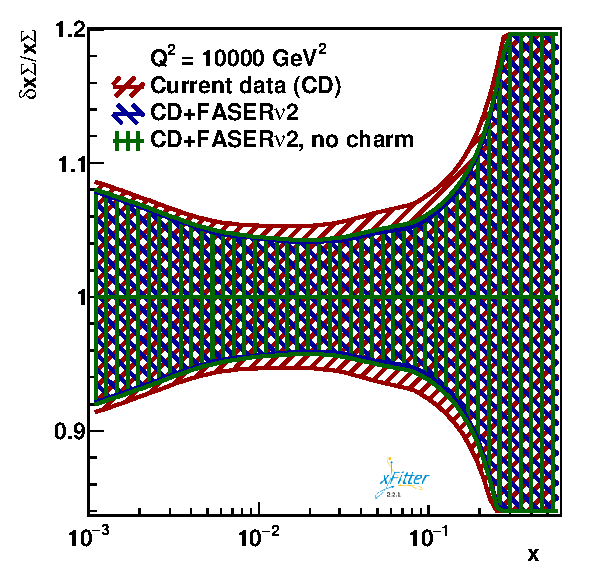
\includegraphics[width=0.32\textwidth]{plots/nuclear_fasernu2/inclusive-only_vs_inclusive+charm/statOnly_FASERv2_q2_10000_pdf_Sea_ratio.pdf}
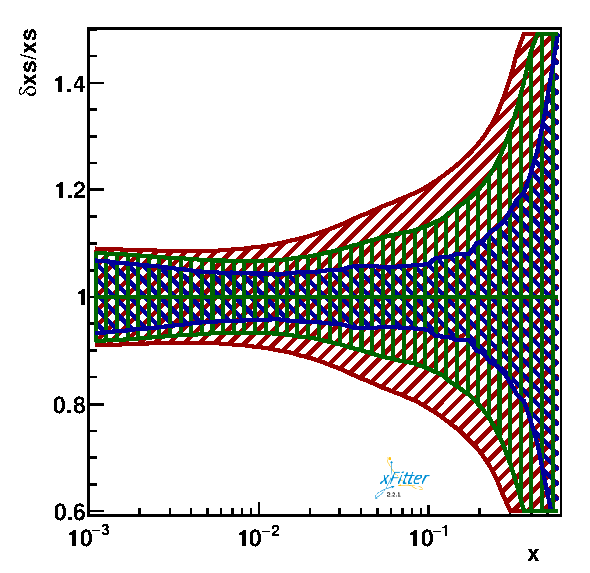
\includegraphics[width=0.32\textwidth]{plots/nuclear_fasernu2/inclusive-only_vs_inclusive+charm/statOnly_FASERv2_q2_10000_pdf_s_ratio.pdf}
\caption{Comparing Fig.~\ref{fig:profiling_baseline_nuclear}, 
to the results obtained without charm production structure functions.
}
\label{fig:profiling_charm_nuclear}
\end{figure}
%%%%%%%%%%%%%%%%%%%%%%%%%%%%%%%%%%%%%%%%%%%%%%%%%%%%%%%%%%%%%%%%%%%%%%%%
%%%%%%%%%%%%%%%%%%%%%%%%%%%%%%%%%%%%%%%%%%%%%%%%%%%%%%%%%%%%%%%%%%%%%%%%
\begin{figure}[t]
\centering
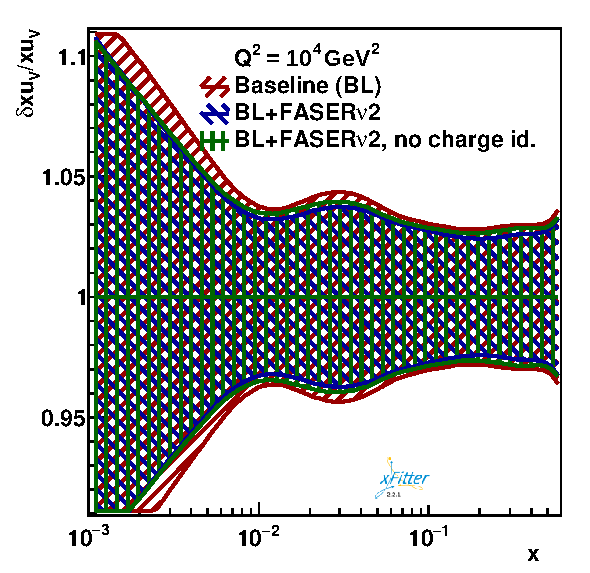
\includegraphics[width=0.32\textwidth]{plots/nuclear_fasernu2/nochargediscrimination/statOnly_FASERv2_q2_10000_pdf_uv_ratio.pdf}
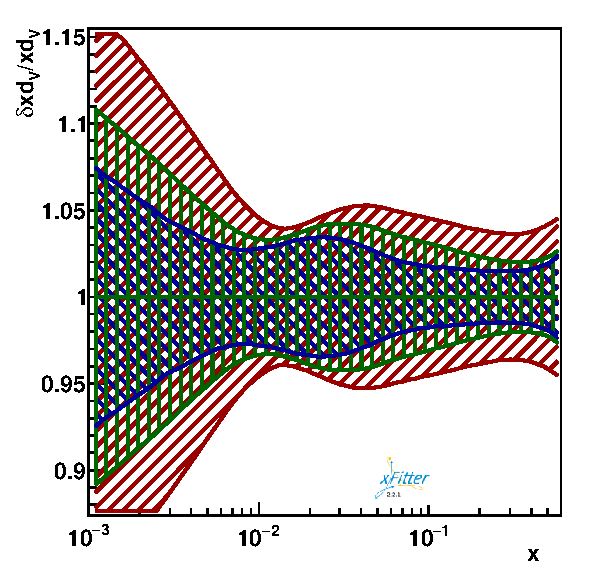
\includegraphics[width=0.32\textwidth]{plots/nuclear_fasernu2/nochargediscrimination/statOnly_FASERv2_q2_10000_pdf_dv_ratio.pdf}
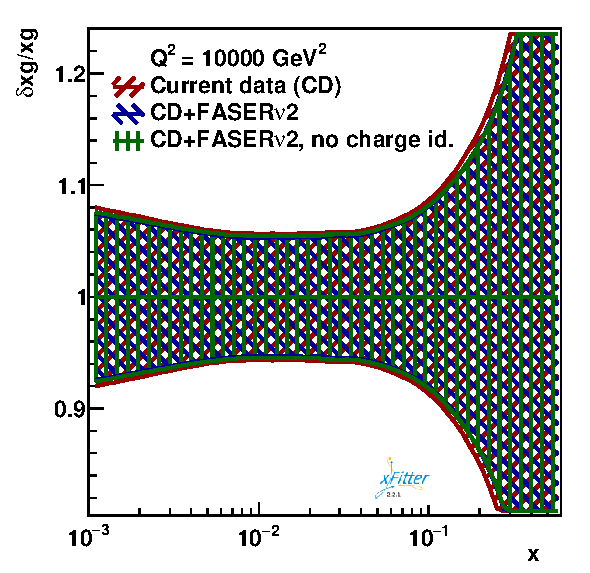
\includegraphics[width=0.32\textwidth]{plots/nuclear_fasernu2/nochargediscrimination/statOnly_FASERv2_q2_10000_pdf_g_ratio.pdf}\\
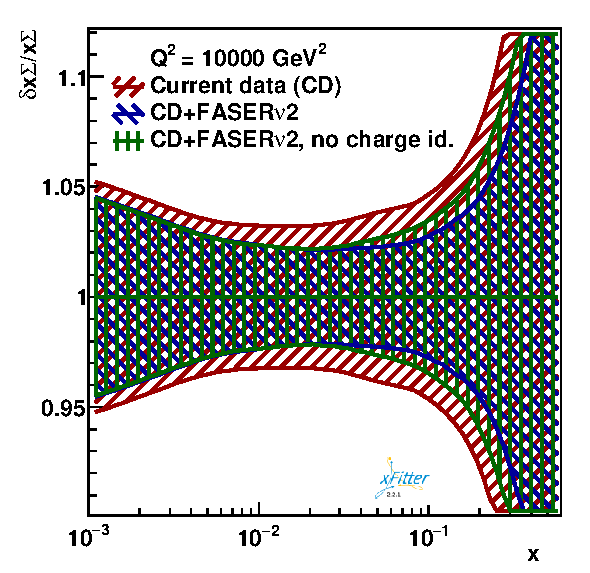
\includegraphics[width=0.32\textwidth]{plots/nuclear_fasernu2/nochargediscrimination/statOnly_FASERv2_q2_10000_pdf_Sea_ratio.pdf}
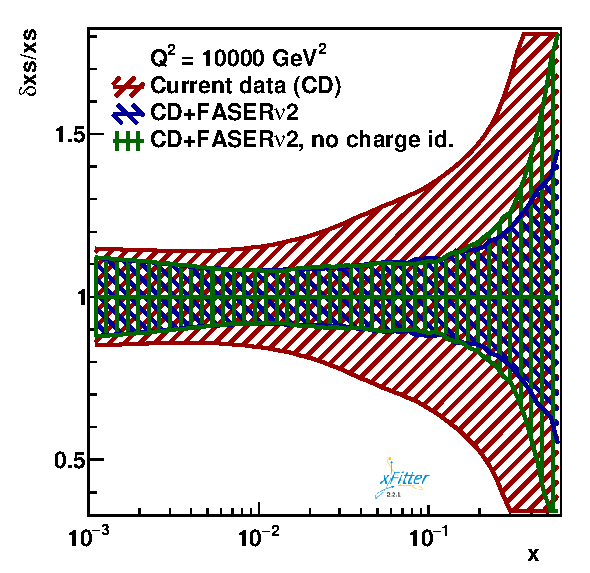
\includegraphics[width=0.32\textwidth]{plots/nuclear_fasernu2/nochargediscrimination/statOnly_FASERv2_q2_10000_pdf_s_ratio.pdf}
\caption{Comparing the results shown in Fig.~\ref{fig:profiling_baseline_nuclear} (red and blue), 
to the results obtained without identifying the charge of the outgoing lepton (green).
}
\label{fig:profiling_nochargediscrimination_nuclear}
\end{figure}
%%%%%%%%%%%%%%%%%%%%%%%%%%%%%%%%%%%%%%%%%%%%%%%%%%%%%%%%%%%%%%%%%%%%%%%%


Plots EPPS21 tungsten target? To quantify size of nuclear modifications?
